\section{Project Plan}
% From the Project Proposal marking sheet:
%   - A well justified, comprehensive, and feasible list of milestones.
%   (with resources and duration).
%   - A complete and accurate risk and/or ethics assessment.

This project would require several milestones to be completed:
\begin{enumerate}
    \item Creating a Proof of Concept (PoC) for VeriTest;
    \item Refining the PoC to be usable in a production setting (November - February).
\end{enumerate}

However, due to the nature of the possible solutions of the framework, it could mean that the details and deadline 
of the milestones could shift dramatically, as each of the solutions (See Sec. \ref{sec:Methodology}) differs in 
their concept. Therefore, each of the milestones would depict several common goals that need to be achieved in order to 
provide value to the project. To illustrate, Fig. \ref{fig:TimelineIsabelleServer}, \ref{fig:TimelineIsabelleScala}, 
and \ref{fig:TimelineDSLInterpreter} have timelines for each of the possible solutions.

Furthermore, it would require a considerable amount of time for me to complete the requirements for the course.
Therefore, the timelines of each milestones should be over-estimated by some factor to allow myself to cope with 
the demands of thesis and other courses requirements. These requirements would be done alongside the project milestones, 
namely:

\begin{enumerate}
    \item Progress Seminar (Due 9 October 2023);
    \item Conference Paper (Due 9 May 2024);
    \item Poster \& Demonstration (Due 17 May 2024);
    \item Thesis Submission (Due 3 June 2024).
\end{enumerate}

\begin{figure}
    \label{fig:TimelineIsabelleServer}
    \centering
    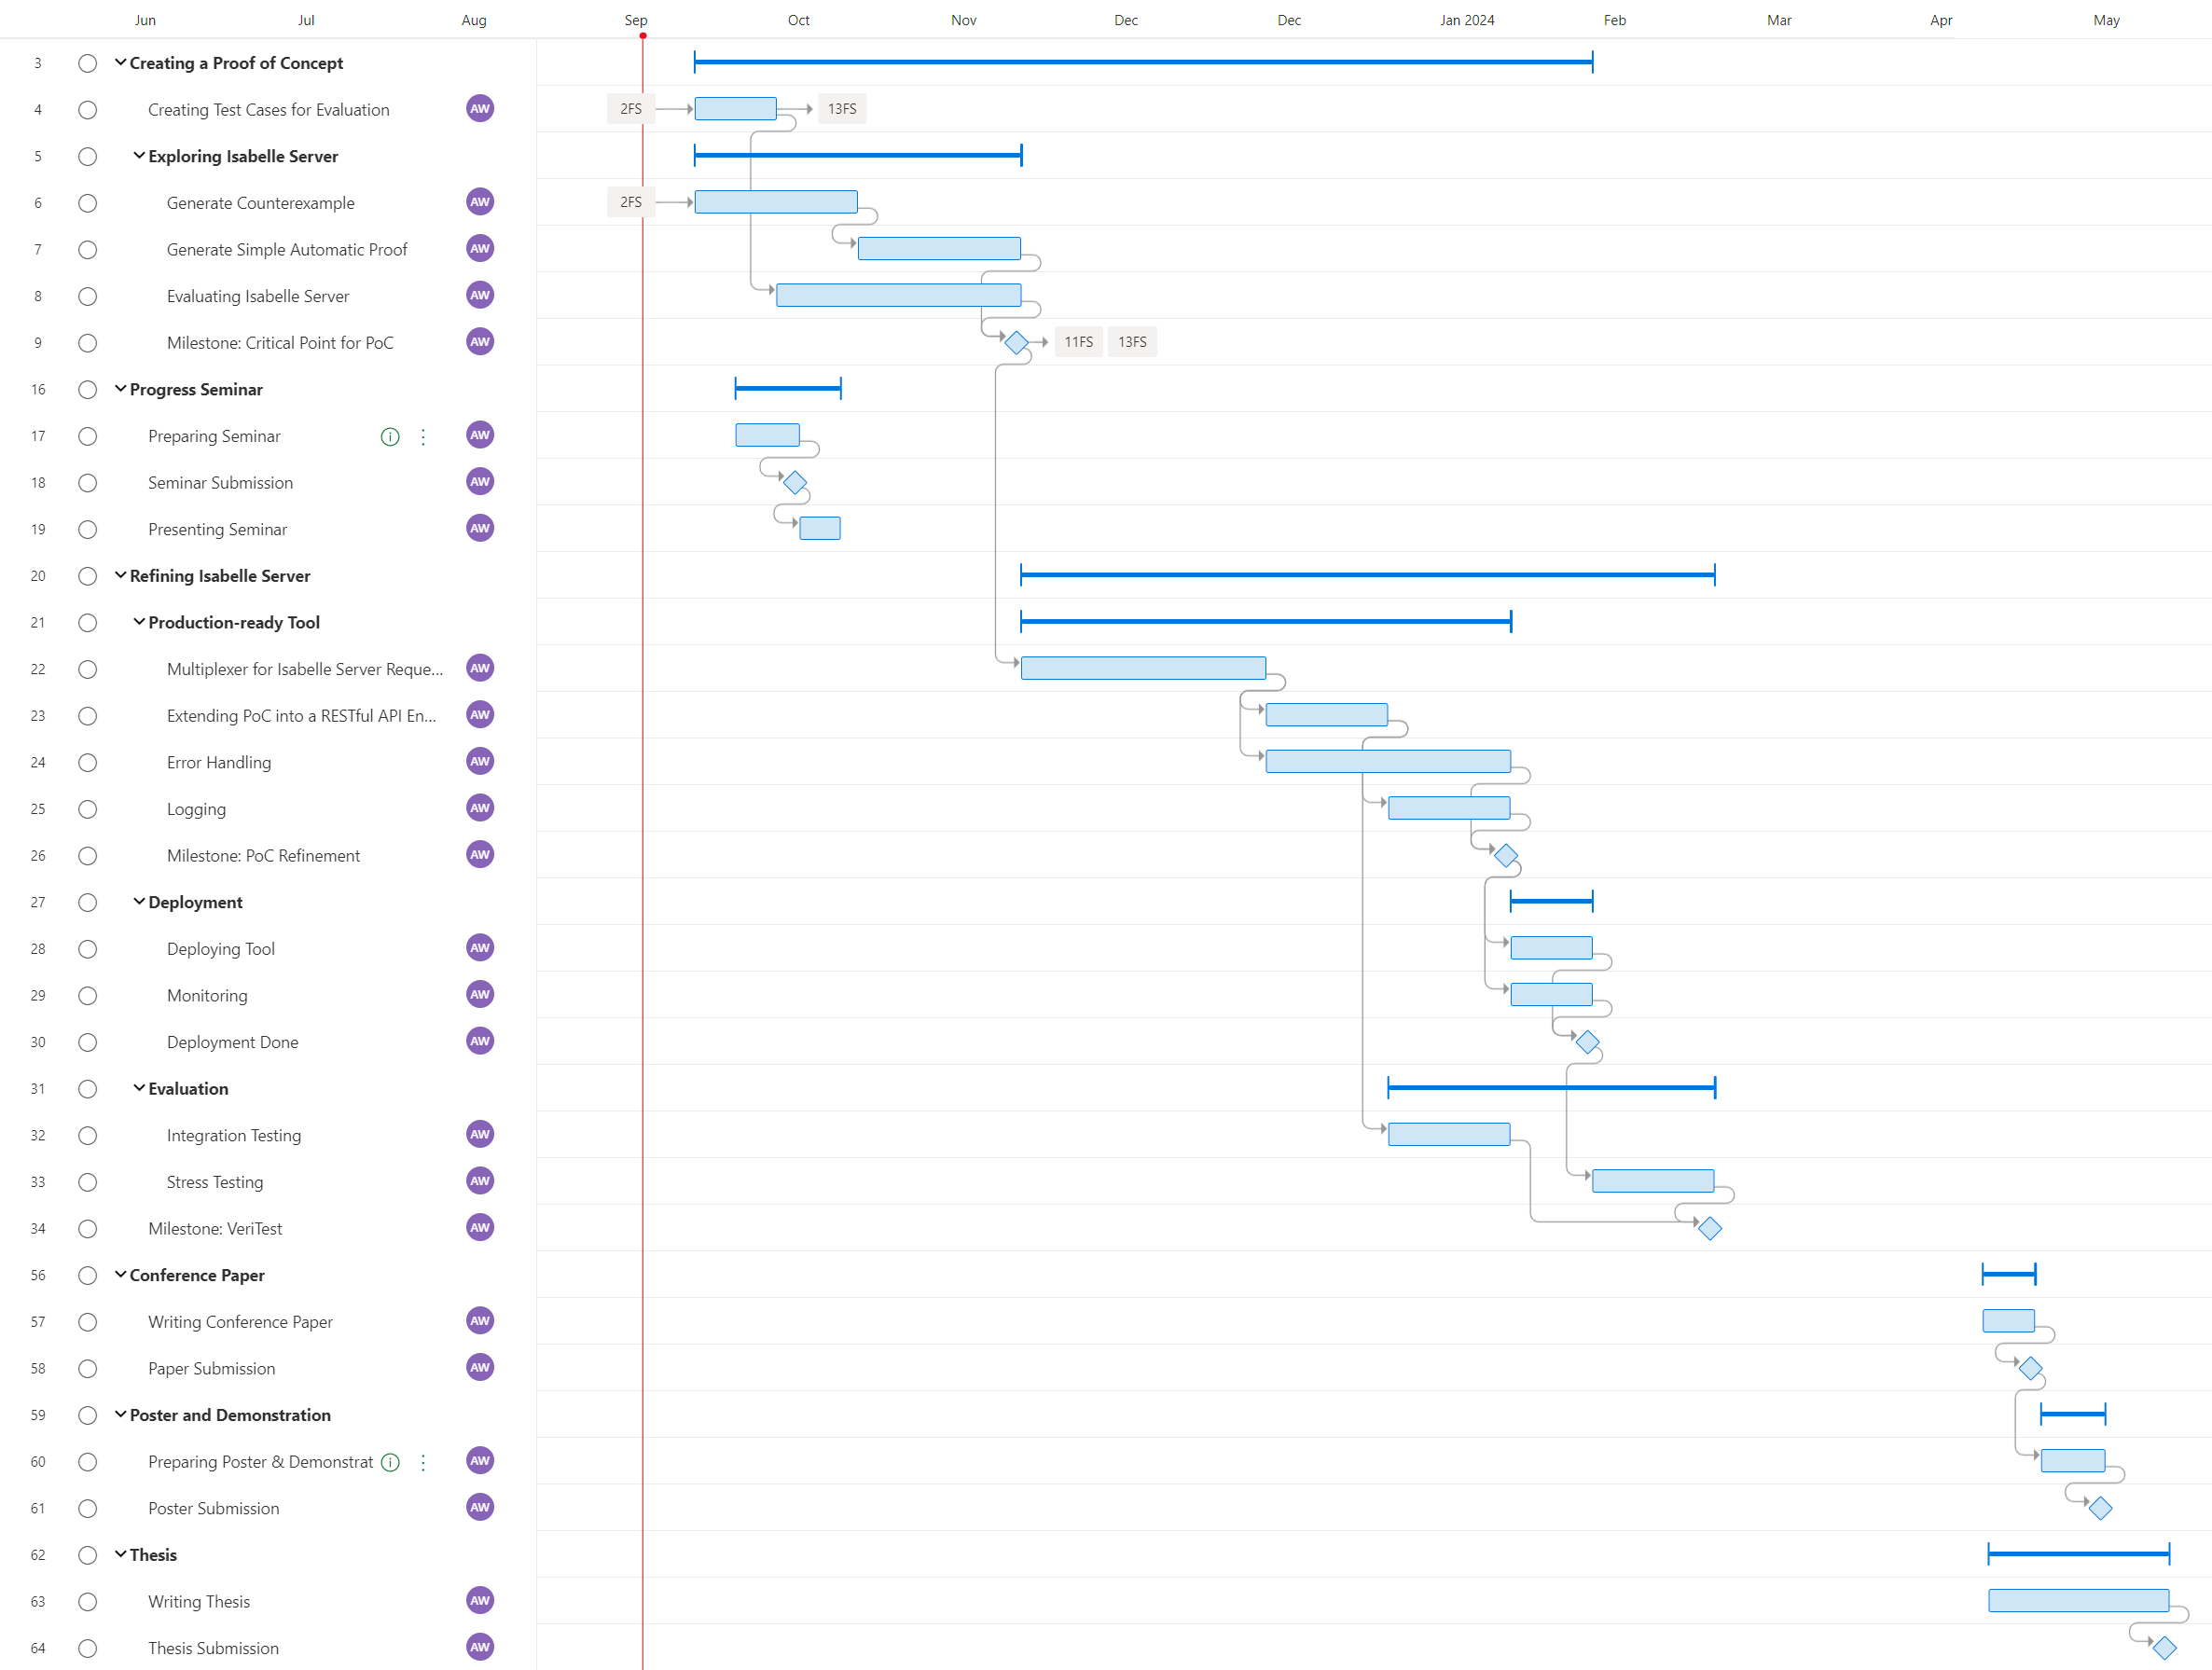
\includegraphics[width=1\textwidth]{timeline-isabelle-server.png}
    \caption{Project timeline for Isabelle Server solution (See Sec. \ref{sec:IsabelleServer})}
\end{figure}

\begin{figure}
    \label{fig:TimelineIsabelleScala}
    \centering
    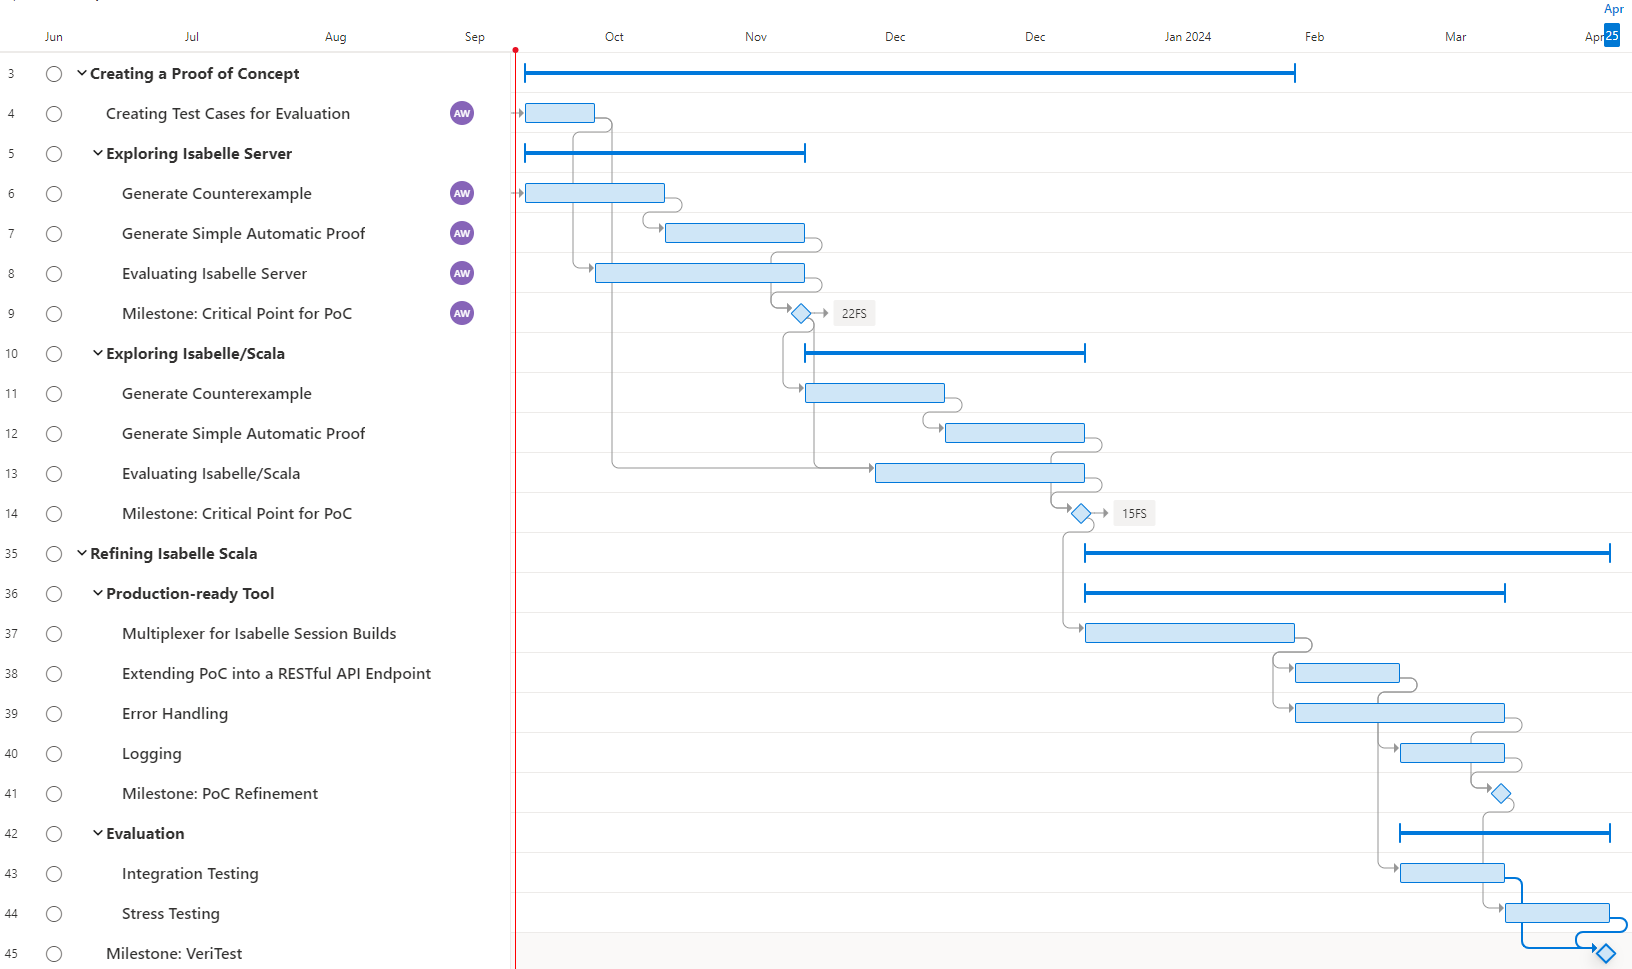
\includegraphics[width=1\textwidth]{timeline-isabelle-scala.png}
    \caption{Project timeline for Isabelle/Scala solution (See Sec. \ref{sec:IsabelleScala})}
\end{figure}

\begin{figure}
    \label{fig:TimelineDSLInterpreter}
    \centering
    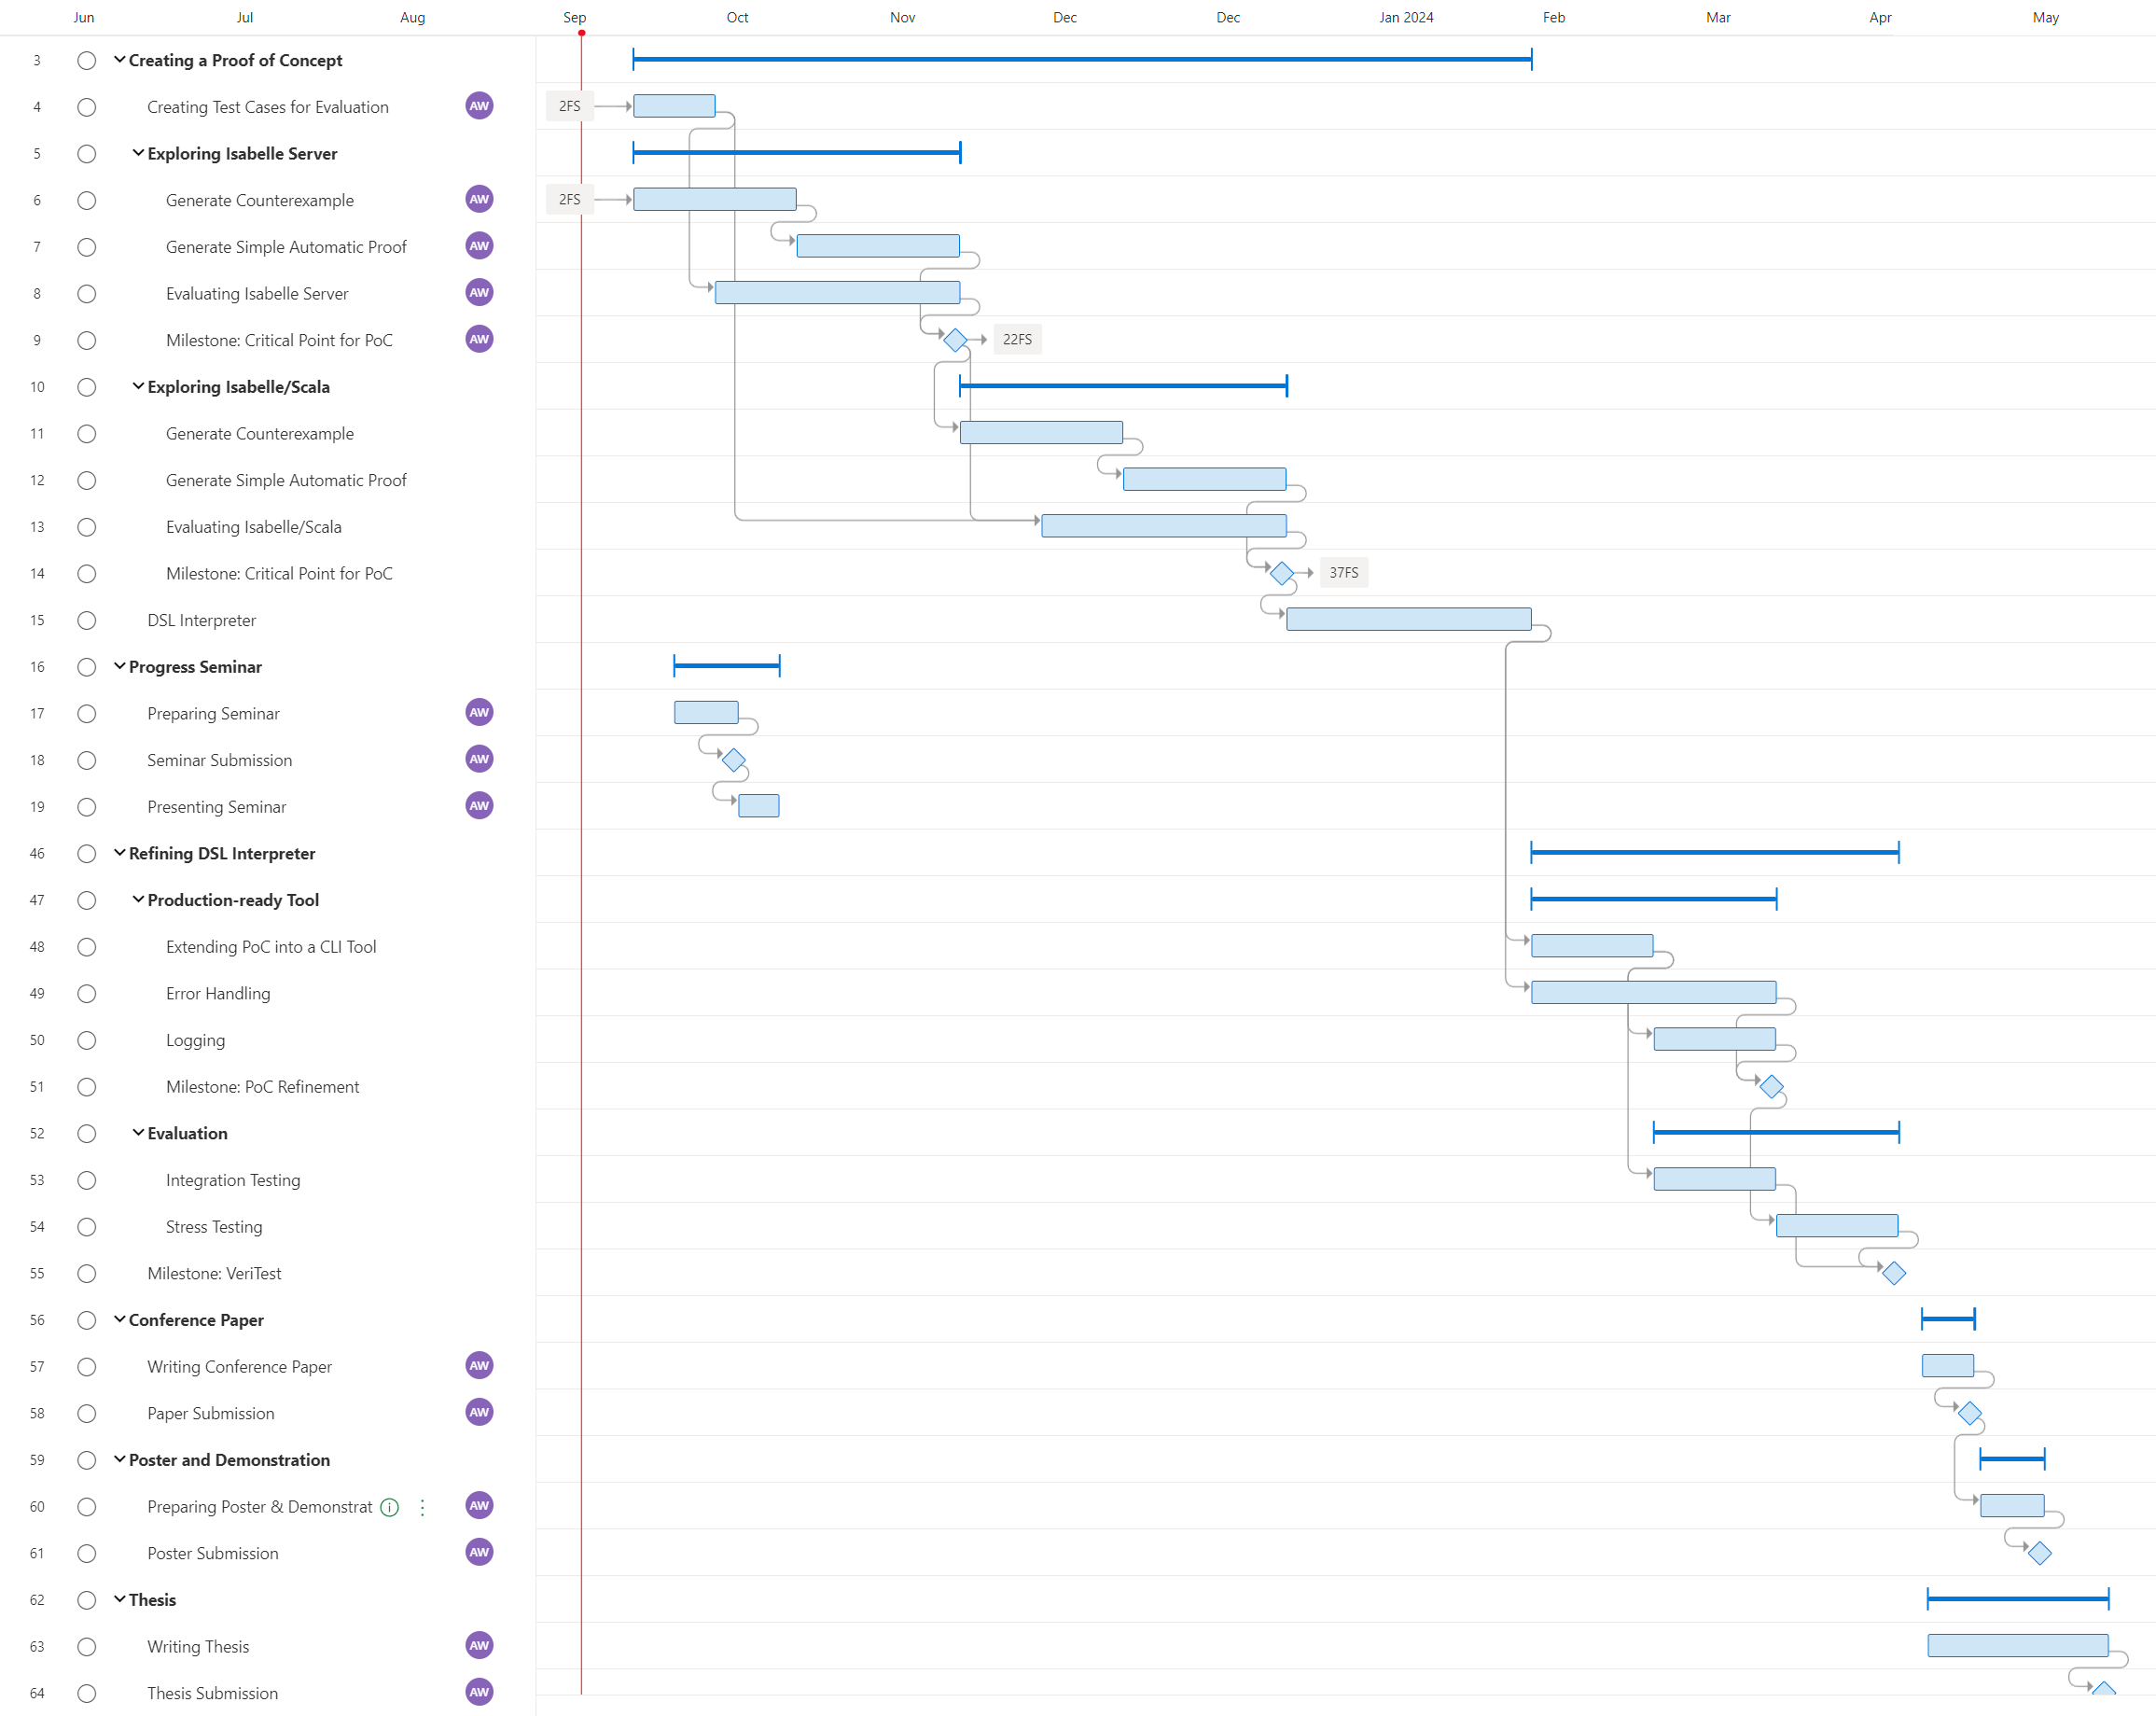
\includegraphics[width=1\textwidth]{timeline-dsl.png}
    \caption{Project timeline for DSL Interpreter solution (See Sec. \ref{sec:DSLInterpreter})}
\end{figure}

\pagebreak

\subsection{Milestones}
\label{sec:Milestones}
% Break your project down into component sub-goals and estimate how long
% you expect each to take.

\subsubsection{Milestone 1: Creating a Proof of Concept}

To create a PoC for solution Isabelle Server (Sec. \ref{sec:IsabelleServer}) and Isabelle/Scala (Sec. \ref{sec:IsabelleScala}), 
the PoC needs to be able to generate counterexamples and simple automatic proofs for an optimization rule. 
The generated proof then can be evaluated by its accuracy. Furthermore, the evaluation will include determining the 
feasibility of the solution.

If both of the solutions are not feasible, then the last resort would be DSL Interpreter (Sec. \ref{sec:IsabelleScala}).
This milestone would represent an extension of Isabelle's \cite{IsabelleHOL} command line interface, and would work on 
the previous knowledge of generating counterexamples and simple automatic proofs from previous solutions. Evaluating this 
solution's milestone would be trivial, as it would build upon the semi-automatic solutions provided in Veriopt 
\cite[Sec. 5.1]{Term_Graph_Optimizations}.

Depending on the feasibility of each solutions, we would have a \emph{critical point} in the timeline where the project 
could decide whether to continue with the solution or not. Fig. \ref{fig:TimelineIsabelleScala} illustrates a critical point 
where \emph{if} the Isabelle Server solution is not feasible, the timeline goes through a different critical path that 
evaluates the feasibility of the Isabelle/Scala solution.

\subsubsection{Milestone 2: Refining the Proof of Concept}

Refining the PoC would have several phases, which could be done in parallel:
\begin{enumerate}
    \item Creating a production-ready service;
    \item Deployment of the service;
    \item Evaluating the service.
\end{enumerate}

The production-ready service will build upon the non-functional requirements of VeriTest (See Fig. \ref{fig:requirements}). 
The evaluation phase refers to Sec. \ref{sec:Evaluation} and evaluates whether the service does indeed meet the 
non-functional requirements.

Each of the consequent solutions after Isabelle Server would have several phases and tasks omitted. This is due to the nature 
of the solutions itself. Isabelle/Scala solution omits the deployment phase, as it does mean that Isabelle Server cannot be 
used to offload some of the processing to external Isabelle session build servers. DSL Interpreter solution omits 
Isabelle session build tasks, as the solution would repeatedly build sessions for each optimization phase. Reaching the 
DSL Interpreter solution would also mean that it would not be feasible to extend the PoC into a RESTful service -- since 
each Isabelle session build takes a considerable amount of time.

\pagebreak

\subsection{Risk Assessment}
% What, if any, risks does your project pose.
% What risks are there to your proposed timeline (technical or otherwise).

\begin{table}[h]
    \centering
    \begin{tabular}{|L{0.25\textwidth}|l|L{0.5\textwidth}|}
        \hline
        \textbf{Risk} & \textbf{Consequence} & \textbf{Mitigation} \\
        \hline\hline
        Complexity of utilizing Isabelle is understated & Critical 
            & This proposal has already outlined the feasibility of each solution and should mitigate the risk. 
            
            Additionally, trimming the scope of the project could be an option, but should be a last resort.

            Furthermore, implementing consistent intervals of monitoring and controlling phase of the project should mitigate the 
            risk considerably. \\
        \hline
        The solution does not meet key non-functional requirements & High
            & Frequent discussions about system specifications and advice on implementation with supervisors. \\
        \hline
        Problems with personal devices, i.e. short-circuited motherboard & Medium
            & Frequent backups to the cloud and utilizing UQ-provided labs for development. \\
        \hline
        Occupational Health and Safety & Low
            & The majority of the development would be done in a low-risk setting. Additionally, following UQ guidelines for 
            workstation ergonomic assessment should lower the risk. \\
        \hline
    \end{tabular}
    \caption{Risk Assessment for VeriTest}
\end{table}

\subsection{Ethics Assessment}
% Are there any ethical considerations involved in your project.
% e.g. do you make use of sensitive or personal information.

Minimal ethical considerations are present in the project, due to the scope of the project only involving 
software.